\documentclass[,man,floatsintext]{apa6}
\usepackage{lmodern}
\usepackage{amssymb,amsmath}
\usepackage{ifxetex,ifluatex}
\usepackage{fixltx2e} % provides \textsubscript
\ifnum 0\ifxetex 1\fi\ifluatex 1\fi=0 % if pdftex
  \usepackage[T1]{fontenc}
  \usepackage[utf8]{inputenc}
\else % if luatex or xelatex
  \ifxetex
    \usepackage{mathspec}
  \else
    \usepackage{fontspec}
  \fi
  \defaultfontfeatures{Ligatures=TeX,Scale=MatchLowercase}
\fi
% use upquote if available, for straight quotes in verbatim environments
\IfFileExists{upquote.sty}{\usepackage{upquote}}{}
% use microtype if available
\IfFileExists{microtype.sty}{%
\usepackage{microtype}
\UseMicrotypeSet[protrusion]{basicmath} % disable protrusion for tt fonts
}{}
\usepackage{hyperref}
\hypersetup{unicode=true,
            pdftitle={Simulation-Based Power-Analysis for Factorial ANOVA Designs},
            pdfauthor={Daniël Lakens~\& Aaron Caldwell},
            pdfkeywords={power analysis, ANOVA, hypothesis test, sample size justification},
            pdfborder={0 0 0},
            breaklinks=true}
\urlstyle{same}  % don't use monospace font for urls
\usepackage{graphicx,grffile}
\makeatletter
\def\maxwidth{\ifdim\Gin@nat@width>\linewidth\linewidth\else\Gin@nat@width\fi}
\def\maxheight{\ifdim\Gin@nat@height>\textheight\textheight\else\Gin@nat@height\fi}
\makeatother
% Scale images if necessary, so that they will not overflow the page
% margins by default, and it is still possible to overwrite the defaults
% using explicit options in \includegraphics[width, height, ...]{}
\setkeys{Gin}{width=\maxwidth,height=\maxheight,keepaspectratio}
\IfFileExists{parskip.sty}{%
\usepackage{parskip}
}{% else
\setlength{\parindent}{0pt}
\setlength{\parskip}{6pt plus 2pt minus 1pt}
}
\setlength{\emergencystretch}{3em}  % prevent overfull lines
\providecommand{\tightlist}{%
  \setlength{\itemsep}{0pt}\setlength{\parskip}{0pt}}
\setcounter{secnumdepth}{0}
% Redefines (sub)paragraphs to behave more like sections
\ifx\paragraph\undefined\else
\let\oldparagraph\paragraph
\renewcommand{\paragraph}[1]{\oldparagraph{#1}\mbox{}}
\fi
\ifx\subparagraph\undefined\else
\let\oldsubparagraph\subparagraph
\renewcommand{\subparagraph}[1]{\oldsubparagraph{#1}\mbox{}}
\fi

%%% Use protect on footnotes to avoid problems with footnotes in titles
\let\rmarkdownfootnote\footnote%
\def\footnote{\protect\rmarkdownfootnote}


  \title{Simulation-Based Power-Analysis for Factorial ANOVA Designs}
    \author{Daniël Lakens\textsuperscript{1}~\& Aaron Caldwell\textsuperscript{2}}
    \date{}
  
\shorttitle{ANOVA Power}
\affiliation{
\vspace{0.5cm}
\textsuperscript{1} Eindhoven University of Technology, The Netherlands\\\textsuperscript{2} Department of Health, Human Performance and Recreation, University of Arkansas, USA}
\keywords{power analysis, ANOVA, hypothesis test, sample size justification\newline\indent Word count: 5000}
\usepackage{csquotes}
\usepackage{upgreek}
\captionsetup{font=singlespacing,justification=justified}

\usepackage{longtable}
\usepackage{lscape}
\usepackage{multirow}
\usepackage{tabularx}
\usepackage[flushleft]{threeparttable}
\usepackage{threeparttablex}

\newenvironment{lltable}{\begin{landscape}\begin{center}\begin{ThreePartTable}}{\end{ThreePartTable}\end{center}\end{landscape}}

\makeatletter
\newcommand\LastLTentrywidth{1em}
\newlength\longtablewidth
\setlength{\longtablewidth}{1in}
\newcommand{\getlongtablewidth}{\begingroup \ifcsname LT@\roman{LT@tables}\endcsname \global\longtablewidth=0pt \renewcommand{\LT@entry}[2]{\global\advance\longtablewidth by ##2\relax\gdef\LastLTentrywidth{##2}}\@nameuse{LT@\roman{LT@tables}} \fi \endgroup}


\usepackage{lineno}

\linenumbers

\authornote{All code used to create this manuscript is
provided in an OSF repository at \url{https://osf.io/xxxxx/}.

Correspondence concerning this article should be addressed to Daniël
Lakens, ATLAS 9.402, 5600 MB, Eindhoven, The Netherlands. E-mail:
\href{mailto:D.Lakens@tue.nl}{\nolinkurl{D.Lakens@tue.nl}}}

\abstract{
Researchers need to design informative studies. When the goal of an
experiment is to test a hypothesis based on a frequentist hypothesis
test it is important to justify the sample size based on the statistical
power of the study. However, researchers are faced with challenges when
they try to calculate power for factorial ANOVA designs. First, current
software solutions are limited as they do not allow power analyses for
more complex designs involving multiple within factors. Second, they
require partial eta-squared or Cohen's f as input, which are not the
most intuitive way to specify predicted effects in an ANOVA, and do not
generalize to different experimental designs. We have created R
functions and an online Shiny app that performs simulations for ANOVA
designs for up to three factors with an unlimited number of levels.
Predicted effects are entered by specifying means, standard deviations,
and correlations (for within factors). The simulation provides a-priori
power analyses for all effects in the ANOVA, and all simple comparisons.
No other software is currently available that allows researchers to so
easily perform power analyses for a wide range of ANOVA designs. The app
plots \emph{p}-value distributions for all tests, and allows researchers
to select a range of options to correct for multiple comparisons. This
tutorial will teach researchers how to perform power analysis for ANOVA
designs, and through simulations illustrate important factors that
determine the statistical power of factorial ANOVA designs.


}

\begin{document}
\maketitle

Statistical power is the probability of observing a statistically
signficant result, given a specified effect size, and assuming there is
a true effect. When a researcher aims to analyze a study based on an
analysis of variance (ANOVA), the sample size of the study should be
justified based on the statistical power of the test. A study has low
power to detect effects the researcher is interested in has a high Type
2 error rate, and leads to a high probability of saying there is no
effect, when there actually is a true effect to be found. Whereas power
analyses for simple comparisons are relatively easy to perform, an
a-priori power analysis for factorial ANOVA designs is a challenge.
Available software solutions do not provide easy options for more
complex designs (e.g., a 2x2x2 design, where the first factor is
manipulated between participants, and the last two factors are
manipulated within participants). Popular software solutions such as
G*power require participants to enter their predictions as Cohen's f or
partial eta squared, which are not the most intuitive ways to specify a
hypothesized pattern of results, and which do not generalize to
different experimental designs.

Here, we demonstrate how to perform power analyses for factorial ANOVA
designs based on simulations. We provide R code and a Shiny app that can
be used to calculate the statistical power based on a predicted pattern
of means, standard deviations, and correlations (for within factors).
Simulating studies, and calculating their \emph{p}-values and effect
sizes, are a useful way to gain a better understanding of the factors
that determine the statistical power of hypothesis tests. After
providing an introduction to statistical power in general, and for the
\emph{F}-test specifically, we will demonstrate how the power of
factorial ANOVA designs depends on the pattern of means across
conditions, the number of factors and levels, and the sample size. We
will also illustrate the importance of controlling Type 1 error rates in
exploratory ANOVA's, and the importance to design studies that have high
power for main effects and interactions in an ANOVA, but also for
follow-up tests for simple effects.

\section{Factors That Determine Power in ANOVA
Designs}\label{factors-that-determine-power-in-anova-designs}

You perform a study in which participants interact with an artificial
voice assistant who sounds either cheerful or sad. You measure how much
80 participants in each condition enjoy interacting with the voice
assistant on a line marking scale (coded continously from -5 to 5) and
observe a mean of 0 in the sad condition, and a means of 1 in the
cheerful condition, with an estimated standard deviation of 2. After
submitting your manuscript for publications, reviewers ask you to add a
study with a neutral control condition to examine whether cheerful
voices increase, or sad voices decrease enjoyment (or both). Depending
on what the mean in the neutral condition is, which sample size would
you need to have a high powered study for the expected pattern or means?
A collaborator suggests to switch from a between design to a within
design, to more efficiently collect the data. Which consequence will
this switching to a within-subject design have on the sample size
planning? Because the effect size in the first study could be considered
\enquote{medium} based on the benchmarks by Cohen (1988), does it make
sense to plan for a \enquote{medium} effect size in either the between
of within ANOVA design? And if you justify the sample size based on the
ANOVA, will the study also have sufficient statistical power for the
simple effects (or vice versa)?

Performing simulation studies is an excellent way to develop intuitions
about these questions. The power in ANOVA designs depends on the pattern
of means, the number of groups, the standard deviation, the correlation
between dependent measures, the alpha level, and the sample size. After
these factors have been specified, a simulation study can be perform to
run the planned statistical test on generated data many times, and
summarize the results. Where analytic power solutions exists in software
such as G*Power for ANOVA designs with up to one within-subject factor,
simulation studies are more flexible (and can for example be used to see
what happens in a 3x3x3 within-subject design). \#Statistical Power When
Comparing Differences Among Group Means Let's consider the initial study
we described above, where two group means are compared. We can test the
difference between two means with a \emph{t}-test of a one-way single
factor ANOVA, and the two tests are mathematically equivalent. Figure
\ref{fig:d-plot} and Figure \ref{fig:eta-plot} visualize the
distribution of Cohen's d and partial eta-squared that should be
observed when there is no effect (grey curves) and when the observed
difference between means equals the true effect. In both figures the
light grey areas under the curve mark the observed results that would
lead to a Type 1 error (observing a statistically significant result if
the null-hypothesis is true) and the dark grey areas under the curve
marks the observed effect sizes that would lead to a Type 2 error. An
observed effect is statistically significant if the observed effect size
is larger than the critical value. Critical values are often expressed
as \emph{t}-values or \emph{F}-values, but can be expressed as effect
sizes (Cohen's d and partial eta-squared), and any observed effect size
larger than the critical effect size will be statistically significant.
The goal of power analysis is to choose a sample size so that the
probability of observing a statistically significant effect for a
specified effect size reaches a desired probability. In both Figures,
88.16\% of the expected effect sizes, if the true effect size is d = 0.5
or \(\eta_p^2\) = 0.0588 and 80 participants in each condition are
collected, will be more extreme than the critical effect size (which is
d = 0.312 or \(\eta_p^2\) = 0.024).

\begin{figure}
\centering
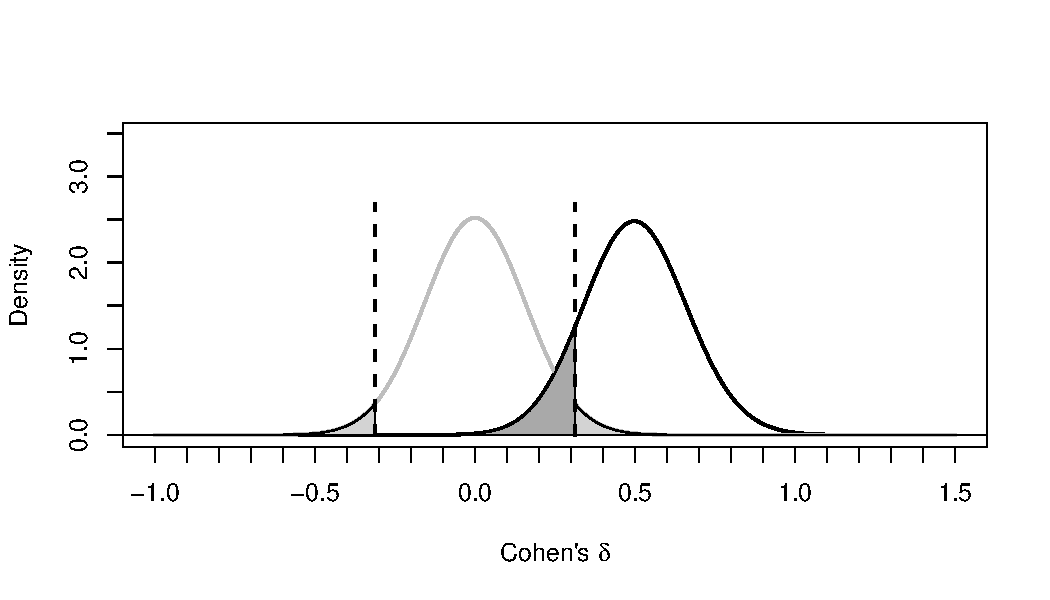
\includegraphics{0.1_Simulation_Based_Power_Analysis_For_Factorial_ANOVA_Designs_files/figure-latex/d-plot-1.pdf}
\caption{\label{fig:d-plot}Distribution of Cohen's d under the
null-hypothesis (grey curve) and alternative hypothesis assuming d = 0.5
(black curve).}
\end{figure}

\begin{figure}
\centering
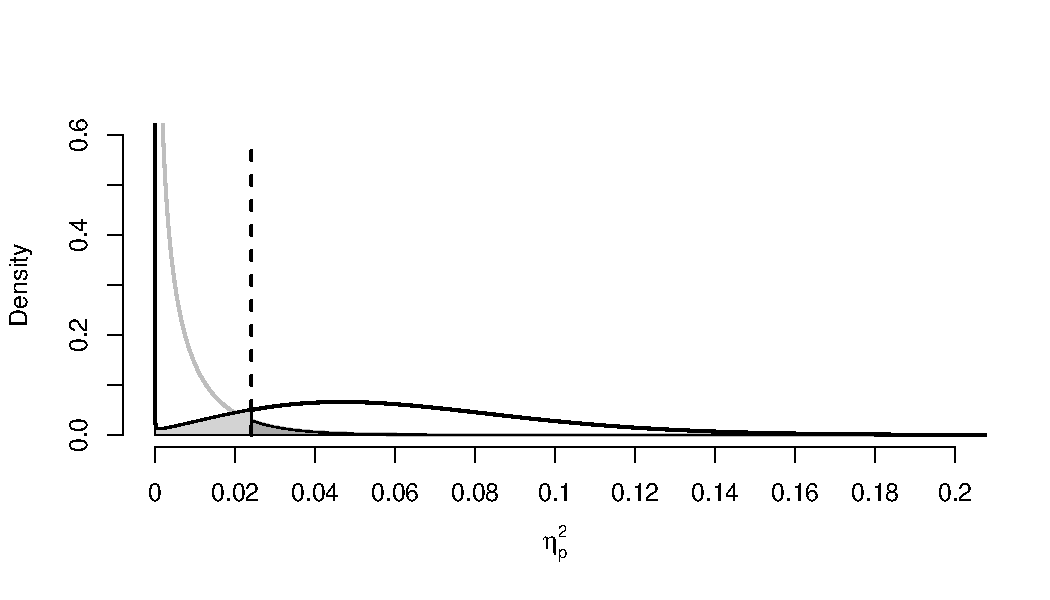
\includegraphics{0.1_Simulation_Based_Power_Analysis_For_Factorial_ANOVA_Designs_files/figure-latex/eta-plot-1.pdf}
\caption{\label{fig:eta-plot}Distribution of eta-squared under the
null-hypothesis (grey curve) and alternative hypothesis assuming partial
eta-squared = 0.0588 (black curve).}
\end{figure}

Two relationships between the \emph{t}-test and the \emph{F}-test when
comparing two means are worth pointing out. First, \(F = t^2\), or the
\emph{F}-value equals the \emph{t}-value, squared. Whereas we typically
think of a \emph{t}-test as the difference between means, the
relationship between the \emph{t}-test and \emph{F}-test reveals that we
can also use the group means to calculate the variance of the difference
between the two means \((m_1 - m_2)^2\). The \emph{F}-test is used to
compute the ratio of the between group variance and the within group
variance, and the between group variance can be used to compare more
than two means. An \emph{F}-value of 1 means the two variances are equal
(as is expected when the null-hypothesis is true) and Cohen's f and
\(\eta_p^2\) would be zero. Second, for two groups the effect size for
an ANOVA, Cohen's f, is half the size of the effect size for
standardized mean differences, Cohen's d, or \(f = \frac{1}{2}d\).
Cohen's d is calculated by dividing the difference between means by the
standard deviation, or

\begin{equation}
d = \frac{m_1-m_2}{\sigma}.
\end{equation}

If we have two groups with means of 1 and 2, and the standard deviation
is 2, Cohen's d is (2-1)/2, or 0.5. Cohen's f is the standard deviation
of the population means divided by the population standard deviation
(Cohen, 1988), or:

\begin{equation}
f = \frac{\sigma _{ m }}{\sigma}
\end{equation}

where for equal sample sizes,

\begin{equation}
\sigma _{ m } = \sqrt { \frac { \sum_ { i = 1 } ^ { k } ( m _ { i } - m ) ^ { 2 } } { k } }.
\end{equation}

Because Cohen's f is an essential part of power power analyses for
factorial ANOVA designs, it is worth illustrating how it is calculated
in an example. If we again take two means of 1 and 2, and a standard
deviation of 2, the grand mean is 1.5. We subtract each condition mean
from the grand mean, take the square, calculate the sum of squares,
divide it by two, and take the square root.
\(\sigma_m = \sqrt{\frac{(1-1.5)^2+(2-1.5)^2}{2}} = \sqrt{\frac{0.25+0.25}{2}} = 0.5\),
and \(f = \frac{0.5}{2} = 0.25.\) We see Cohen's f is half as large as
Cohen's d. Power analyses for ANOVA are based on Cohen's f, but popular
power anaysis software such as G*Power (Faul, Erdfelder, Lang, \&
Buchner, 2007) also allows researchers to specify the effect size as
partial eta-squared (\(\eta_p^2\)). Partial eta-squared can be converted
into Cohen's f:

\begin{equation}
f = \sqrt{\frac{\eta_p^2}{1-\eta_p^2}}
\end{equation}

and Cohen's f can be converted into partial eta-squared:

\begin{equation}
\eta_p^2 = \sqrt{\frac{f^2}{f^2+1}}
\end{equation}

In the example above, \(\eta_p^2 = 0.25^2/(0.25^2+1) = 0.0588\). To
calculate the statistical power assuming a specific true effect size we
need the noncentrality parameter of the distribution. In both Figure
\ref{fig:d-plot} and Figure \ref{fig:eta-plot} we see examples of the
non-central \emph{t}-distribution and non-central \emph{F}-distribution,
or the shape of the expected test statistics when there is a true
effect. Power calculations rely on the nonceptrality parameter (often
referred to as lambda, or \(\lambda\)). Based on \(\lambda\) (which
specifies the shape of the expected distribution) and the critical test
statistic (which specifies the part of the distribution that is more
extreme than the test statistic needed for a statistically significant
test result) we can calculate how often, in the long run, we can expect
test results that will be statistically significant.

\section{Simulating Statistical Power for Different Factorial
Designs}\label{simulating-statistical-power-for-different-factorial-designs}

We have created R code and a Shiny app that simulate factorial ANOVA
designs. At the core, the code generates data for each condition in the
design, performs the test, and calculates the percentage of significant
results and average effect size of all main effects and interactions, as
well as all simple effects. It requires specifying the design of the
study in a string of numbers (for the levels in each factor) and letters
(a \enquote{b} for between factors or \enquote{w} for within factors).
Our initial study above is a \enquote{2b} or two level between subject
design. For ease of interpreting the simulation results, the factors and
levels can be named (for our example, Condtion, cheerful, sad). The
planned sample size should be specified, which is 80 participants in
each between subjects condition. The means for each condition should be
specified (0 and 1), as well as the standard deviation (2). For within
designs the correlation between variables should be specified. With
these variables specified, the design is set up for the simulation. For
a visual confirmation of the input, a figure is created that displays
the means (see Figure \ref{fig:means-plot}).

\begin{figure}
\centering
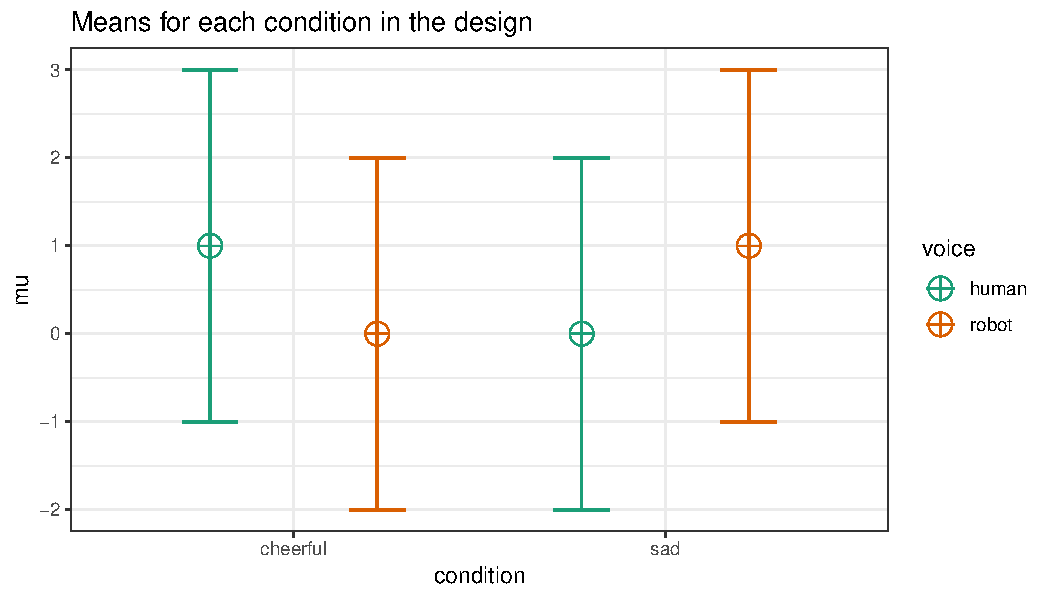
\includegraphics{0.1_Simulation_Based_Power_Analysis_For_Factorial_ANOVA_Designs_files/figure-latex/mean-plot-1.pdf}
\caption{\label{fig:mean-plot}Vizualization for the expected means and
confidence intervals for each condition.}
\end{figure}

The results of a simulation study will vary each time the simulation is
performed (but can be made reproducible by specifying a \enquote{seed}
number). Results become more stable, the more simulations are performed,
but the simulations also take longer. The functions that performs the
simulation requires specifying the number of simulations, the alpha
level for the tests, and any adjustment for multiple comparisons for the
ANOVA. If 100.000 simulations are performed in R with a seed set to 2019
(these settings will be used for all simulation results in this
manuscript), we see the statistical power (based on the percentage of
\emph{p} \textless{} \(\alpha\) results) is 80 and the average effect
size is 0.05. The simulation also provides the results for the simple
effects, based on \emph{t}-tests comparing each group. Since there are
only two groups in this example, the results for the statistical power
are identical, but the effect size is -0.45, which is the effect size in
Cohen's d. Now the basic idea behind the simulation is clear, we can
start exploring how changing the experimental design influences our
power. We will first examine what happens if we add a third condition to
the design. Let's assume we expect the neutral voice condition to fall
either between the cheerful and sad conditions, or perhaps to be equal
to the cheerful condition (based on the idea that the sad voice leads to
less enjoyment, but the cheerful voice does not lead to more enjoyment).
The design now has 3 between subject conditions, and we can explore what
happens if we would collect 80 participants in each condition.

If we assume the mean falls exactly between between the cheerful and sad
conditions the simulations show the statistical power for our design is
reduced to 70, and the effect size is 0.06. If we assume the mean the
mean is equal to the cheerful condition, the power increases to 100.
Compared to the two group design, three things have changed. First, an
additional group was added to the design, which increases the numerator
degrees of freedom, which makes the non-central \emph{F}-distribution
more similar to the central \emph{F}-distribution, and reduces the
statistical power. Second, the total sample size is 50\% larger, which
increases the statistical power. Third, the effect size has decreased,
which reduces the statistical power. The exact effect of these three
changes on the statistical power is difficult to predict. The most
important conclusion based on these simuations is that when the design
is changed, one can not assume the effect size remains unchanged.

What happens if we would perform the second study as a
within-participants design? Instead of collecting three groups of
participants, we only collect one group, and let this group evaluate the
cheerful, neutral, and sad voice assistants. The sample size needed in a
within-design (NW), relative to the sample needed in between-design
(NB), is (from Maxwell \& Delaney, 2004, p.~562, formula 47):

\begin{equation}
N_{W}=\frac{N_{B}(1-\rho)}{a}
\end{equation}

Here \emph{a} is the number of within-subject levels, \(\rho\) is the
correlation between the measurements, and the formula assumes normal
distributions and compound symmetry, and ignores the difference in
degrees of freedom between the two types of tests, so it is a rough (but
useful) approximation. Whenever the correlation between dependent
measures is positive, the sample size that is needed in a
within-participants condition will be smaller than the requires sample
size for a between-participants condition.

We need to be able to estimate the correlation between the dependent
variables we can expect. Ideally, this estimate will be based on data
from previous experiments. If we plan to collect 80 participants, and
assume the correlation between all dependent variables is 0.5, the power
for the repeated-measures ANOVA is 100. Note that simulation studies
allow for great flexibility, and the Shiny app also allows researchers
to enter a correlation matrix specifying the expected correlation
between each individual pair of measurements, instead of assuming the
correlations between dependent variables are identical for all pairs.

\section{Power for Interactions and Simple
Effects}\label{power-for-interactions-and-simple-effects}

The effect size for an ANOVA design depends on the pattern of means.
Let's assume the researcher aims to perform a follow-up test to examine
the effect of a second factor on the enjoyment of interacting with an
artificial voice assistant. In addition to making the voice sound
cheerful or sad, a second factor is introduced by making the voice sound
more robotic compared to the default human-like voice. Different
patterns of results could be expected. Either the same effect is
observed for robotic voices, or no effect is observed for robotic
voices, or the opposite effect is observed for robotic voices (a
\enquote{Marvin-the-Depressed-Robot-Effect}). In the first case, we will
only observe a main effect of voice, but in the other two scenarios
there is an interaction effect between human-likeness of the voice and
the emotional tone of the voice. We can start by simulating the power
for a cross-over interaction for a 2x2 between-participant design with
80 participants in each group.

\begin{figure}
\centering
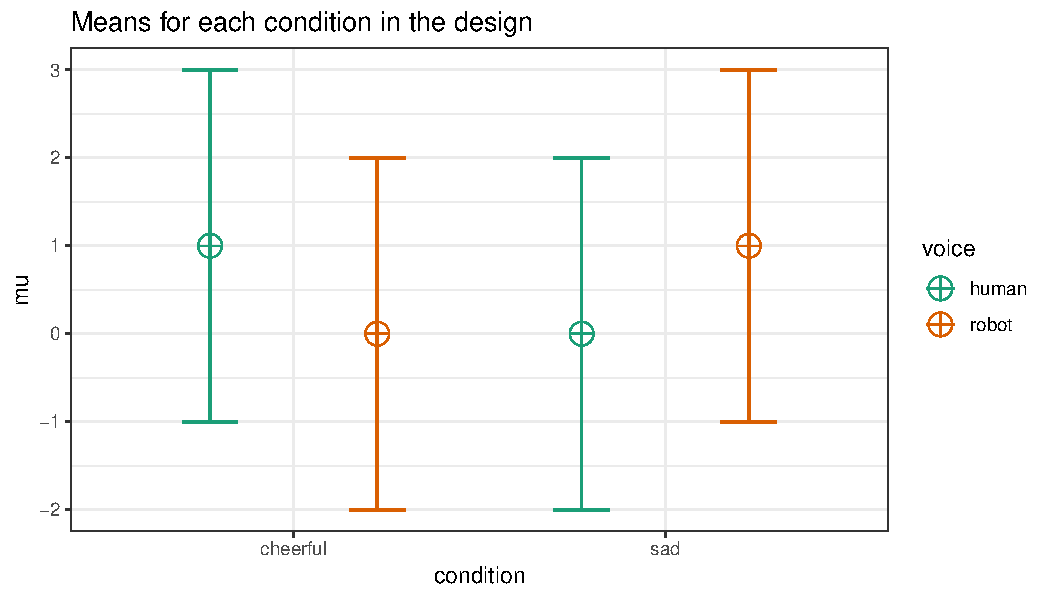
\includegraphics{0.1_Simulation_Based_Power_Analysis_For_Factorial_ANOVA_Designs_files/figure-latex/mean-plot_2-1.pdf}
\caption{(\#fig:mean-plot\_2)Expected means and confidence intervals for
each of the four conditions.}
\end{figure}

Mathematically the interaction effect is computed as the cell mean minus
the sum of the grand mean, the marginal mean in row i minus the grand
mean, and the marginal mean in column j minus grand mean. For example,
for the cheerful human-like voice condition this is 1 (the value in the
cell) - (0.5 {[}the grand mean{]} + 0.5 {[}the cell mean minus the
marginal mean in row 1, 0.5{]} + 0.5 {[}the cell mean minus the marginal
mean in column 2, 0.5{]}). 1 - (0.5 + (0.5) + (0.5)) = -0.5. Completing
this for all four cells gives the values -0.5, 0.5, 0.5, -0.5. Cohen's f
is then
\(f = \frac { \sqrt { \frac { -0.5^2 + 0.5^2 + 0.5 + -0.5^2 } { 4 } }}{ 2 } = 0.25\).
Cohen's f for the 2x2 design is the same as for the two-group design,
but we have collected twice as many people in total (4 times 80).
Simulations show we have would have exactly the same power for a
cross-over (or sometimes called \enquote{disordinal}) interaction is we
halved the sample size per group from 80 to 40. Main effects in an ANOVA
are based on the mean averaged over the other factors (e.g., the main
effect of human-like versus robot-like voice, irrespective of whether it
is cheerful or sad). The interaction effect, which can be contrast coded
as 1, -1, -1, 1, is similarly a test of whether the effects are
non-additive based on the scores in each cell, where the null-hypothesis
of no additive effect can be rejected if the deviation expected when
effects in each cell would be purely additive can be rejected. The key
insight here is that the total sample size determines the power (cf.
Westfall (2015)).

We can also examine what the statistical power would be if the pattern
of results indicated that there was no difference in interacting with a
cheerful of sad conversational agent with a robot voice. In this case,
we expect an \enquote{ordinal} interaction (the means for the human-like
voice are never lower than the means for the robot-like voice, and thus
there is no cross-over effect). The pattern of means is now 1, 0, 0, 0.
As has been pointed out (Giner-Sorolla, 2018; Simonsohn, 2014) these
designs require larger samples to have the same power to detect the
interaction compared to the two-group comparison. The reason for this is
that the effect size is only half as large, with Cohen's f = 0.125
(compared to 0.25 in the cross-over interaction). To achieve the same
power as for the two-group comparison, a total sample size of 635 is
required, almost four times as large as the sample size for the
two-group comparison.

The power in the 2x2 ordinal interaction where only one cell mean
differs from the other three cell means is identical to the power we
would have if the single mean was twice as far from the remaining means
(for a pattern of means of 2, 0, 0, 0). Similarly, if we would examine a
2x2x2 interaction where only one cell differs from the other means,
Cohen's f would be 0.25 only when the pattern of means is 4, 0, 0, 0, 0,
0, 0, 0 across the eight cells.\\
The key insight here is that the effect size, and thus the power, for
interactions in ANOVA designs depends on the pattern of the means. A
\enquote{medium} effect size translates into a much more extreme pattern
of means in an ordinal interaction than in a disordinal (crossover)
interaction, or in a 2x2x2 interaction compared to a 2x2 interaction.
For this reason, it is not very intuitive to start a power analysis
based on an assumption of the effect size. The same effect size can
represent very different patterns of means depending on the type of
interaction and the number of factors. Instead, it might be more
intuitive to think about the pattern of means that you expect, and
compute the corresponding Cohen's f.

\section{Power for Within Designs}\label{power-for-within-designs}

One feature of the simulation is that it provides the statistical power
for all tests that can be performed is calculated, including simple
effects. Throughout the examples above, as long as the means are 1 and
0, all simple effects either compare means that are identical (and thus
only Type 1 errors are observed) or that have an effect size of d = 0.5
(for between designs).

\newpage

\section{References}\label{references}

\setlength{\parindent}{-0.5in} \setlength{\leftskip}{0.5in}

\hypertarget{refs}{}
\hypertarget{ref-cohen_statistical_1988}{}
Cohen, J. (1988). \emph{Statistical power analysis for the behavioral
sciences} (2nd ed.). Hillsdale, N.J: L. Erlbaum Associates.

\hypertarget{ref-faul_gpower_2007}{}
Faul, F., Erdfelder, E., Lang, A.-G., \& Buchner, A. (2007). GPower 3: A
flexible statistical power analysis program for the social, behavioral,
and biomedical sciences. \emph{Behavior Research Methods}, \emph{39}(2),
175--191.
doi:\href{https://doi.org/10.3758/BF03193146}{10.3758/BF03193146}

\hypertarget{ref-giner-sorolla_powering_2018}{}
Giner-Sorolla, R. (2018, January). Powering Your Interaction.
\emph{Approaching Significance}.

\hypertarget{ref-simonsohn_no-way_2014}{}
Simonsohn, U. (2014, March). No-way Interactions. \emph{Data Colada}.

\hypertarget{ref-westfall_think_2015}{}
Westfall, J. (2015, May). Think about total N, not n per cell.
\emph{Cookie Scientist}.


\end{document}
